%%%%%%%%%%%%%%%%%%%%%%%%%%%%%%%%%%%%%%%%%%%%%%%%%%%%%%%%%%%%%%%%%%%%%%%%%%%%%%%%%%%%%%%%%%%%%%%%%%%%%%%%%%%%%%%
\documentclass[a4paper,timesnewroman,12pt,twoside]{report}
%\usepackage[utf8]{inputenc}
\usepackage[a4paper]{geometry}
\geometry{verbose,tmargin=1in,bmargin=1in,lmargin=1.25in,rmargin=1in}
\usepackage{authblk,lineno,hyperref,color,lscape,url,sectsty}
\usepackage[autostyle]{csquotes}
\usepackage[dvipsnames]{xcolor}
\usepackage[labelfont=bf]{caption}
\usepackage{emptypage}
\usepackage{array,float,multirow,graphicx,setspace,cite,url,titlesec,tocloft}
%\usepackage{mathrsfs}
\usepackage{}
\usepackage{amsmath,cleveref,amsfonts,mathtools,notoccite}
\usepackage{chngcntr,rotating,pdflscape,enumitem,algpseudocode,algorithm,subcaption}
\usepackage{calligra}
\numberwithin{equation}{section}
\linespread{1.3}
\titleformat{\chapter}[display]
%{\normalfont\huge \bfseries}{\chaptertitlename\ \thechapter}{5pt}{\Huge}
{\normalfont \huge \filleft \bfseries\color{black}}{\chaptertitlename\ \thechapter}{8pt}{\LARGE}
\titlespacing*{\chapter}{0pt}{0pt}{10pt}
\graphicspath{{./Figures/}}
\renewcommand\cftaftertoctitle{\par\noindent\rule{\textwidth}{2pt}\par\vskip-3.5em}
\renewcommand\cftafterloftitle{\par\noindent\rule{\textwidth}{2pt}\par\vskip-3.0em}
\renewcommand\cftafterlottitle{\par\noindent\rule{\textwidth}{2pt}\par\vskip-3.0em}
% Line spacing
\usepackage{setspace}
\linespread{1.2} % �� slightly reduced (looks like your reference)

% Graphics
\usepackage{graphicx}
\usepackage{subcaption}
\graphicspath{{./Figures/}}
\usepackage{float}
\usepackage{placeins}

% Colors & links
\usepackage[dvipsnames]{xcolor}
\usepackage{hyperref}
\usepackage{float}

% Math
\usepackage{amsmath,amsfonts,amssymb}

% Tables
\usepackage{array}
\usepackage{multirow}
\usepackage{longtable}

% Lists
\usepackage{enumitem}

% Algorithms
\usepackage{algorithm}
\usepackage{algpseudocode}

% Remove titlesec (�� IMPORTANT — avoids spacing issues)
% \usepackage{titlesec}


% Captions
\usepackage[labelfont=bf]{caption}

% Empty pages
\usepackage{emptypage}
\usepackage[breaklinks]{hyperref}
\usepackage{xurl}

\begin{document}

%%%%%%%%%%%%%%%% FRONT MATTER %%%%%%%%%%%%%%%%

\pagenumbering{roman}

\thispagestyle{empty}
\graphicspath{{Figures/PNG/}{Figures/}}

\begin{center}

\vspace{8mm}

\huge \textcolor{blue}{\textbf{Airline Reservation System }} \\


\vspace{8mm}

\Large \textit{A Field project report submitted by}

\vspace{5mm}

\renewcommand{\arraystretch}{1.3}
\begin{tabular}{c c}
\textbf{\Large B. Dhanush} & {\large (241FA18429)} \\
\textbf{\Large P. Bhanu Teja Reddy} & {\large (241FA18435)} \\
\textbf{\Large A. Rohith Srinivasa Reddy} & {\large (241FA18440)} \\
\textbf{\Large Sk. Salman} & {\large (241FA18451)} \\
\end{tabular}

\vspace{5mm}

\large \textit {in partial fulfillment for the award of the degree of}

\vspace{6mm}

\Large {\textbf{\textcolor{violet}{BACHELOR OF TECHNOLOGY}}}

\vspace{2mm}

\large in

\vspace{3mm}

\textbf{{\emph \large {\textcolor{black}{Artificial Intelligence \& Machine Learning}}}}

\vspace{5mm}

{\large \textit {Under the Guidance of}}

\vspace{2mm}

\Large \textbf{\textcolor{black} {Mr P.Srinivasa Rao(Asst.professor)}}}

\vspace{5mm}

% �� No floating figure now

\includegraphics[height=2.5cm,width=8cm]{Figures/vfstr.jpg}

\vspace{3mm}

\large { 
\textbf{ \textcolor{violet}{Department of Advanced Computer Science and Engineering}\\
\textcolor{black}{\textit{School of Computing and Informatics}}}\\
\textbf{\textcolor{black}{Vignan’s Foundation for Science, Technology \& Research}}} \\

(Deemed to be University) \\
Andhra Pradesh-522213, India \\

\vspace{3mm}

\textbf{April-2026}

\end{center}

\thispagestyle{empty}
\clearpage

\pagenumbering{gobble}

\begin{figure}[h!]
    \centering
    
\includegraphics[width=0.35\linewidth]{Figures/vfstr.jpg}
\end{figure}

\linespread{1.2}

\begin{center}
{\large \textbf{\textcolor{violet}{Department of Advanced Computer Science and Engineering}}} \\[2mm]
{\large \textbf{School of Computing and Informatics}} \\[1mm]
{\textbf{Vignan's Foundation for Science, Technology \& Research}} \\[1mm]
(Deemed to be University) \\[1mm]
{\textbf{Andhra Pradesh, India-522213}}
\end{center}

\vspace{4mm}
\noindent\rule{\linewidth}{1.5pt}

\vspace{6mm}

\begin{center}
{\bf\Large CERTIFICATE}
\end{center}

\vspace{4mm}


This is to certify that the project entitled 
\textcolor{violet}{\textbf{“Airline Reservation System Using Object-Oriented Programming”}} 
is being submitted by B. Dhanush (241FA18429), Bhanu Teja Reddy P (241FA18435), 
A. Rohith (241FA18440), and Sk. Salman (241FA18451), in partial fulfilment of the 
requirements for the award of the degree of Bachelor of Technology in Computer Science 
and Engineering, Department of Advanced Computer Science and Engineering, Vignan’s 
Foundation for Science and Technology and Research (Deemed to be University), Vadlamudi, 
Guntur District, Andhra Pradesh, India.

\vspace{4mm}

\noindent
This is a bonafide record of the work carried out by them under my guidance and supervision.

\vspace{20mm}
\begin{center}
\renewcommand{\arraystretch}{1.5}
\begin{tabular}{>{\centering\arraybackslash}p{6cm} >{\centering\arraybackslash}p{6cm}}

\textbf{Guide} & \textbf{HOD, ACSE} \\[10pt]

Mr. P. Srinivasa Rao & Dr. D. Radha Rani \\

\end{tabular}
\end{center}
\addcontentsline{toc}{chapter}{Certificate}
\clearpage

\pagenumbering{gobble}

\begin{figure}[h!]
    \centering
    
\includegraphics[width=0.5\linewidth]{Figures/vfstr.jpg}
\end{figure}

\linespread{1.3}

\begin{center}
{\large \textbf{\textcolor{violet}{Department of Advanced Computer Science and Engineering}}} \\
{\large \textbf{School of Computing and Informatics}} \\
{\textbf{Vignan's Foundation for Science, Technology \& Research}} \\
(Deemed to be University) \\
{\textbf{Andhra Pradesh, India-522213}}
\end{center}

\noindent\rule{\linewidth}{2pt}

\begin{center}
{\bf\Large DECLARATION} \\
\vspace{5mm}
\end{center}

We hereby declare that the project work titled 
\textbf{“Airline Reservation System Using Object-Oriented Programming”} 
submitted by us is a bonafide work carried out under the guidance of 
\textbf{P.Srinivasa Rao}, Department of Advanced Computer Science and Engineering, 
Vignan’s Foundation for Science, Technology and Research (Deemed to be University), 
Vadlamudi, Guntur, Andhra Pradesh.

We further declare that this work has not been submitted previously for the award of any degree or diploma in any university or institution.

\vspace{20mm}

\begin{flushright}
\begin{tabular}{>{\raggedleft\arraybackslash}m{10cm}}

\MakeUppercase{B. Dhanush} \\
(241FA18429) \\[15pt]

\MakeUppercase{P.Bhanu Teja Reddy} \\
(241FA18435) \\[15pt]

\MakeUppercase{A. Rohith Srinivasa Reddy} \\
(241FA18440) \\[15pt]

\MakeUppercase{Sk. Salman} \\
(241FA18451) \\[15pt]

\end{tabular}
\end{flushright}

\addcontentsline{toc}{chapter}{Declaration}
\clearpage

\vspace{-6.0\baselineskip}
\textbf{\begin{flushright}
		{\LARGE \textbf{ACKNOWLEDGMENTS}}
\end{flushright}}
\vspace{-0.5\baselineskip}
\noindent\rule{\linewidth}{2pt}
w
\par First and foremost, we express our sincere gratitude to the \textbf{ALMIGHTY GOD} for giving us strength and guidance to complete this project successfully.\\

\par We are grateful to our beloved founder and chairman \textbf{Dr. Lavu Rathaiah} for providing us the opportunity to pursue our B.Tech at Vignan’s Foundation for Science, Technology and Research.\\

\par We extend our sincere thanks to our respected Vice Chancellor(i/c) \textbf{Dr. K. V. Krishna Kishore} and Registrar \textbf{Dr. P. M. V. Rao} for their continuous support.\\

\par We express our gratitude to \textbf{Dr. Venkatesulu Dondeti}, Addl. Dean and Professor, Department of ACSE, for his valuable encouragement.\\

\par We are thankful to \textbf{Dr. D. Radha Rani}, Head of the Department, ACSE, for her guidance and support.\\

\par We feel privileged to express our sincere thanks to our guide, \textbf{Mr. P. Srinivasa Rao}, Assistant Professor, Department of ACSE, for her continuous guidance, support, and valuable suggestions throughout the project.\\

\par We also thank \textbf{Dr. Amar Jukuntla}, Project Coordinator, for his support and encouragement.\\

\par Finally, we express our heartfelt thanks to all faculty members, friends, and family for their constant support and motivation.

\addcontentsline{toc}{chapter}{Acknowledgments}
\clearpage

\chapter*{ABSTRACT}
\addcontentsline{toc}{chapter}{ABSTRACT}
\noindent\rule{\linewidth}{2pt}

\vspace{0pt}

\vspace{30pt}

\noindent
The rapid growth of the aviation industry has increased the demand for efficient and reliable airline reservation systems. Traditional manual booking methods are often time-consuming, error-prone, and inefficient when handling large volumes of passenger data and flight schedules. To address these challenges, this project presents the design and development of an Airline Reservation System using Object-Oriented Programming (OOP) in Java.

\par
The proposed system provides a user-friendly platform that enables passengers to search for flights, check seat availability, book tickets, cancel reservations, and view booking history. The system is developed using Java for application logic and MySQL for database management, with JDBC used for seamless connectivity between the application and the database.

\par
The implementation of OOP concepts such as encapsulation, inheritance, abstraction, and polymorphism ensures modularity, scalability, and maintainability of the system. Encapsulation is used to protect sensitive data, inheritance supports code reusability, abstraction simplifies complex operations, and polymorphism enables flexible functionality.

\par
The system ensures real-time updates of seat availability and maintains accurate passenger and booking records. It reduces manual errors and improves the efficiency of reservation management. The results demonstrate that the proposed system provides a reliable and efficient solution for airline ticket booking and management.

\par
This project highlights the practical application of Object-Oriented Programming in solving real-world problems and lays the foundation for future enhancements such as online payment integration, web-based interfaces, and cloud deployment.
\clearpage

\tableofcontents
\clearpage

%%%%%%%%%%%%%%%% MAIN CONTENT %%%%%%%%%%%%%%%%

\pagenumbering{arabic}

\chapter{Introduction}
\noindent\rule{\linewidth}{2pt}
This chapter provides a brief description of the Airline Reservation System, including its background, motivation, problem statement, and the overall organization of the project report.

\section{Background}

The airline industry plays a significant role in modern transportation by enabling efficient travel across cities, countries, and continents. With the increasing demand for air travel, airlines must manage large volumes of passenger data, flight schedules, and booking operations. Traditional manual reservation systems are often inefficient, time-consuming, and prone to human errors.

An Airline Reservation System is a software application designed to automate the process of flight booking, seat allocation, and passenger management. It allows users to search for flights, check seat availability, book tickets, and cancel reservations. The use of automated systems improves accuracy, reduces manual effort, and enhances customer satisfaction.

\section{Motivation for the present research work}

The motivation behind this project arises from the limitations of manual and semi-automated reservation systems. These systems often lead to booking conflicts, incorrect passenger records, and inefficient seat allocation. As the number of air travelers continues to increase, there is a growing need for reliable and efficient reservation systems.

This project aims to develop an Airline Reservation System using Object-Oriented Programming (OOP) in Java. The goal is to design a system that is modular, scalable, and easy to maintain, while providing accurate and fast booking services.

\section{Problem statement}

In the current digital era, managing airline reservations efficiently is a significant challenge for many organizations. Existing systems may lack proper structure, scalability, and data consistency, leading to issues such as double booking, incorrect data handling, and delays in processing.

The problem addressed in this project is to design and develop an automated Airline Reservation System that ensures accurate booking management, efficient seat allocation, and secure handling of passenger data.

\section{Organization of the project report}

The research work presented in this report is organized into several chapters:

\begin{itemize}
\item \textbf{Chapter 1} describes the introduction, including background, motivation, and problem statement.
\item \textbf{Chapter 2} presents the literature review of existing systems.
\item \textbf{Chapter 3} explains the methodology used in the development of the system.
\item \textbf{Chapter 4} describes the system architecture.
\item \textbf{Chapter 5} discusses the implementation details.
\item \textbf{Chapter 6} presents results and analysis.
\item \textbf{Chapter 7} concludes the project and suggests future enhancements.
\end{itemize}
\clearpage

\chapter{Literature Review}
\noindent\rule{\linewidth}{2pt}
This chapter presents a review of recent research works related to airline reservation systems, focusing on automation, database management, and object-oriented system design. It helps in understanding current challenges and identifying gaps that motivate the proposed system.

\section{Literature Review}

\subsection{Cloud-Based Airline Reservation System (2023)}

This study focuses on developing a cloud-based airline reservation system that supports real-time booking and scalability. The system improves availability and performance by leveraging cloud infrastructure. It highlights the importance of distributed systems in handling large volumes of airline data efficiently.

\subsection{Java-Based Airline Reservation System Using OOP (2023)}

This research presents an airline reservation system developed using Java and Object-Oriented Programming principles. The study emphasizes modular design using encapsulation, inheritance, and polymorphism. It improves system maintainability and reduces code complexity.

\subsection{Web-Based Airline Booking System with Real-Time Updates (2022)}

This paper proposes a web-based airline reservation system that provides real-time flight availability and booking confirmation. The system ensures efficient seat management and reduces booking conflicts through database synchronization.

\subsection{Role-Based Airline Reservation System (2022)}

This study introduces a role-based access control system for airline reservations. It defines different user roles such as admin, staff, and passengers. The system enhances security and ensures controlled access to system functionalities.

\subsection{Database Optimization Techniques in Reservation Systems (2021)}

This research focuses on improving database performance in reservation systems using indexing and normalization techniques. It highlights how optimized database design reduces query time and improves system efficiency.

\subsection{Integration of Online Payment Systems in Airline Booking (2024)}

This paper discusses the integration of secure online payment gateways in airline reservation systems. It emphasizes transaction security, user authentication, and real-time payment confirmation to enhance user experience.

\subsection{AI-Based Flight Recommendation System (2025)}

This study introduces the use of Artificial Intelligence to recommend flights based on user preferences and historical data. It improves user satisfaction by providing personalized flight suggestions.

\subsection{Mobile-Based Airline Reservation Application (2024)}

This research focuses on developing a mobile application for airline reservations. It provides features such as flight search, booking, and notifications, improving accessibility and user convenience.

\subsection{Secure Airline Reservation System Using Encryption (2023)}

This paper highlights the importance of data security in airline systems. It implements encryption techniques to protect user data and booking information, ensuring system reliability.

\subsection{Scalable Microservices-Based Reservation System (2025)}

This study proposes a microservices architecture for airline reservation systems. It improves scalability, fault tolerance, and system performance by dividing the system into independent services.

\section{Summary}

From the reviewed literature, it is observed that modern airline reservation systems focus on scalability, real-time processing, security, and user experience. However, many systems lack proper implementation of structured Object-Oriented Programming concepts. This gap motivates the development of the proposed Airline Reservation System using Java and OOP principles to ensure modularity, maintainability, and efficiency.
\clearpage

\chapter{Methodology}
\noindent\rule{\linewidth}{2pt}
This chapter describes the methodology adopted for the design and development of the Airline Reservation System, including the system overview, development approach, technologies used, workflow, and modules of the system.

\section{Overview}

The Airline Reservation System is designed to automate the process of booking and managing airline tickets. The system is developed using Object-Oriented Programming (OOP) concepts in Java, ensuring modularity and maintainability. It provides functionalities such as user registration, flight search, ticket booking, cancellation, and booking history management.

\section{System Development Approach}

The system is developed using a structured approach consisting of the following phases:

\begin{itemize}
\item \textbf{Requirement Analysis:} Identification of system requirements such as user authentication, flight search, booking, and cancellation.

\item \textbf{System Design:} Designing system architecture, class diagrams, and database schema.

\item \textbf{Implementation:} Developing the system using Java and integrating it with MySQL using JDBC.

\item \textbf{Testing:} Verifying system functionality and fixing errors to ensure smooth operation.
\end{itemize}

\section{Technologies Used}

The following technologies are used in the development of the system:

\begin{itemize}
\item \textbf{Programming Language:} Java
\item \textbf{Database:} MySQL
\item \textbf{Connectivity:} JDBC
\item \textbf{Development Tools:} Eclipse / IntelliJ IDEA
\end{itemize}

\section{System Workflow}

The workflow of the system describes how users interact with the application:

\begin{enumerate}
\item User registers or logs into the system.
\item User searches for flights based on source and destination.
\item System displays available flights.
\item User selects a flight and books a ticket.
\item System updates seat availability and stores booking details.
\item User can cancel bookings if required.
\item User can view booking history.
\end{enumerate}

\section{Modules of the System}

The system is divided into the following modules:

\begin{itemize}
\item \textbf{User Module:} Handles user registration and login.

\item \textbf{Flight Module:} Manages flight details and availability.

\item \textbf{Booking Module:} Handles ticket booking and confirmation.

\item \textbf{Cancellation Module:} Manages ticket cancellation and seat updates.

\item \textbf{Admin Module:} Allows management of flights, users, and bookings.
\end{itemize}

\section{Summary}

This chapter presented the methodology used for developing the Airline Reservation System. It explained the development approach, technologies used, workflow, and system modules, ensuring a structured and efficient system design.
\clearpage


\chapter{System Architecture}
\noindent\rule{\linewidth}{2pt}
This chapter describes the overall system architecture of the Airline Reservation System. It explains how different components interact with each other to provide efficient and reliable booking services.

\section{System Architecture Diagram}

The Airline Reservation System follows a layered architecture consisting of three main layers: Presentation Layer, Application Layer, and Database Layer.
\begin{figure}[h!]
\centering
\includegraphics[width=0.9\textwidth]{ACSE_Project_Template_Field_Projects (1)/Figures/syss.jpeg}
\caption{System Architecture of Airline Reservation System}
\end{figure}

\section{Description of Architecture}

The system is designed using a three-layer architecture to ensure modularity and efficient data management.

The \textbf{Presentation Layer} is responsible for user interaction. It provides a console-based or graphical user interface through which users can search flights, book tickets, and manage reservations.

The \textbf{Application Layer} contains the core logic of the system. It is implemented using Java and includes classes such as Passenger, Flight, Booking, and Admin. This layer processes user requests and performs operations like booking, cancellation, and data validation.

The \textbf{Database Layer} stores all system data including user details, flight information, and booking records. MySQL is used as the database, and JDBC is used to connect the application with the database.

\section{System Workflow Diagram}

The workflow of the system describes the sequence of operations performed during the reservation process.

\begin{enumerate}
\item User registers or logs into the system.
\item User searches for flights by entering source and destination.
\item System displays available flights.
\item User selects a flight and proceeds to booking.
\item System checks seat availability.
\item If seats are available, booking is confirmed.
\item System updates database and displays confirmation.
\item User can cancel booking if required.
\end{enumerate}

\section{System Workflow Description}

The workflow begins when a user logs into the system. The user searches for flights based on travel details. The system retrieves available flights from the database and displays them to the user. After selecting a flight, the system checks seat availability. If seats are available, booking details are stored in the database, and confirmation is provided to the user.

If the user chooses to cancel a booking, the system updates the database and increases seat availability accordingly.

\section{Database Design}

The database is designed to manage all system data efficiently. It consists of multiple tables that store user, flight, and booking information.

\begin{itemize}
\item \textbf{Users Table:} Stores user details such as user ID, name, email, and password.
\item \textbf{Flights Table:} Contains flight information including flight ID, source, destination, timing, and available seats.
\item \textbf{Bookings Table:} Stores booking details such as booking ID, user ID, flight ID, and status.
\end{itemize}

\section{Summary}

This chapter presented the system architecture of the Airline Reservation System. It explained the layered architecture, workflow of the system, and database design. The architecture ensures efficient communication between different components and supports scalability and maintainability.
\clearpage

\chapter{Implementation}
\noindent\rule{\linewidth}{2pt}
\section{Introduction}

This chapter presents the implementation of the Airline Reservation System developed using Java. The system is console-based and demonstrates various functionalities such as user registration, login, flight booking, and cancellation. The implementation focuses on providing a user-friendly interface and efficient handling of airline operations.

\section{System Interface}

\subsection{Main Menu}

The main menu acts as the entry point of the system, allowing users to navigate through different functionalities. It provides options for both administrators and passengers to access the system.

\begin{figure}[H]
\centering
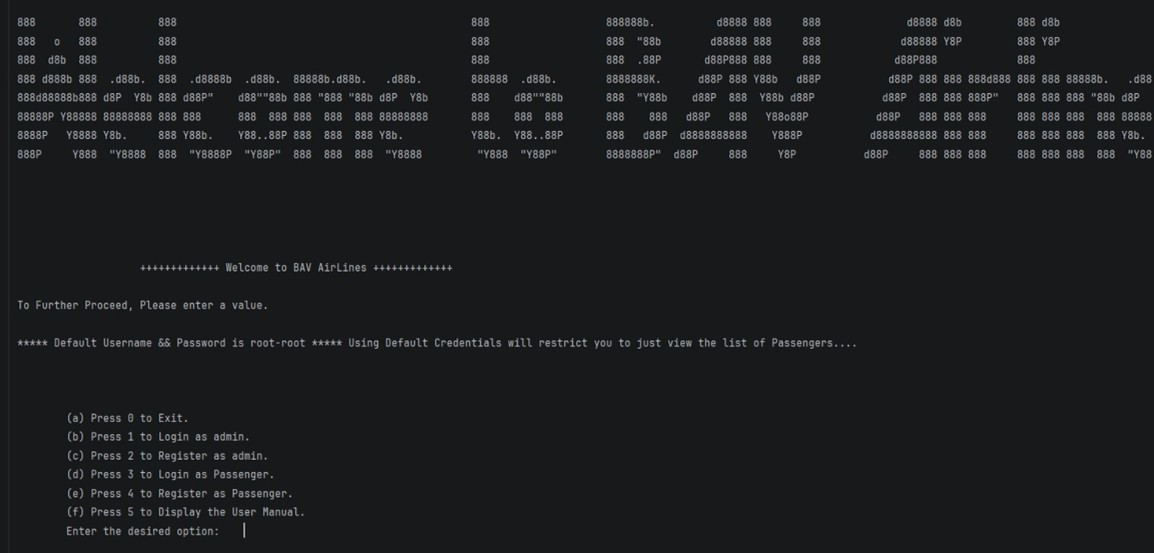
\includegraphics[width=\textwidth]{Figures/homepage.jpg}
\caption{Main Menu of Airline Reservation System}
\end{figure}
\vspace{-5pt}



As shown in Figure~5.1, the main menu provides options such as admin login, passenger login, registration, and access to the user manual. This menu ensures smooth navigation and improves user interaction with the system.

\FloatBarrier

\subsection{User Registration}

The user registration module enables new users to create an account by entering the required personal details.

\begin{figure}[H]
\centering
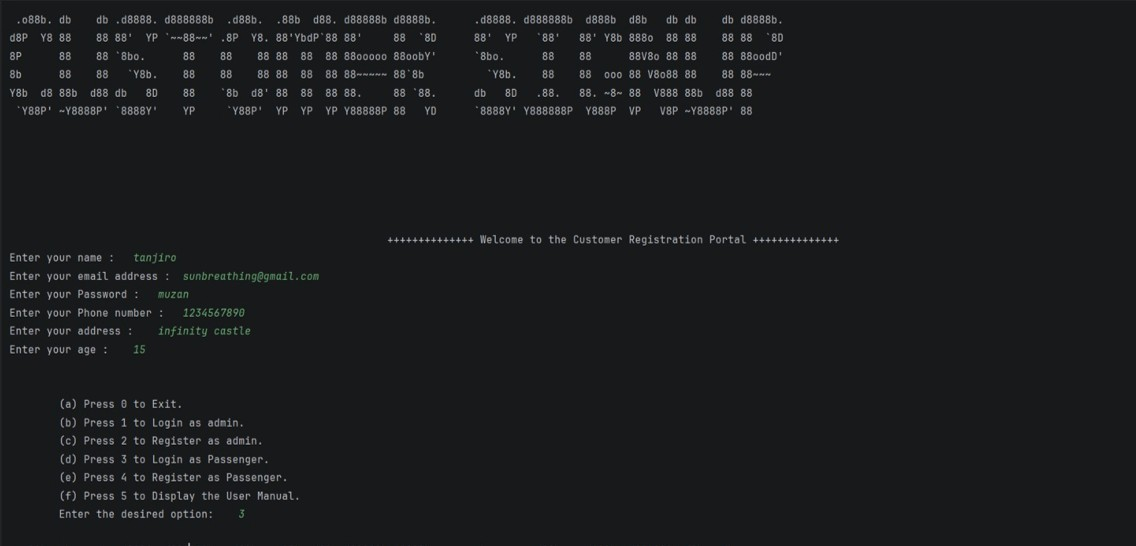
\includegraphics[width=\textwidth]{Figures/Picture2.jpg}
\caption{User Registration Interface}
\end{figure}
\vspace{-5pt}

As illustrated in Figure~5.2, the system collects essential user information such as name, email, password, phone number, and address. This module ensures secure and organized storage of user data for future login and booking operations.

\FloatBarrier

\section{Flight Management}

\subsection{Flight Schedule Display}

The flight schedule module provides users with detailed information about available flights.

\begin{figure}[H]
\centering
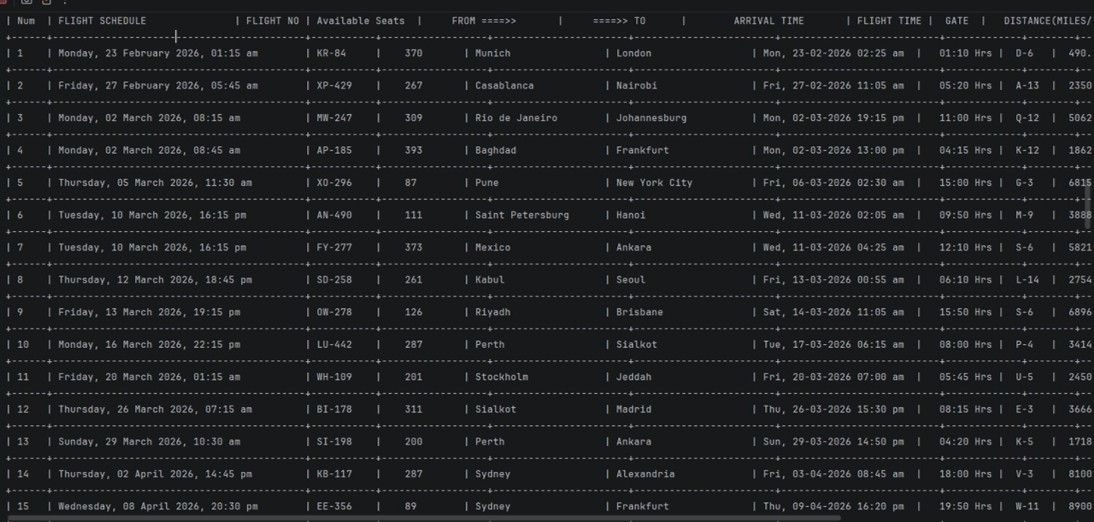
\includegraphics[width=\textwidth]{Figures/Picture4.jpg}
\caption{Flight Schedule Display}
\end{figure}
\vspace{-5pt}

Figure~5.3 shows the list of available flights along with important details such as flight number, available seats, departure location, destination, arrival time, and flight duration. This helps users make informed decisions while booking tickets.

\FloatBarrier

\subsection{Ticket Booking}

The ticket booking module allows users to reserve seats based on their preferences.

\begin{figure}[H]
\centering
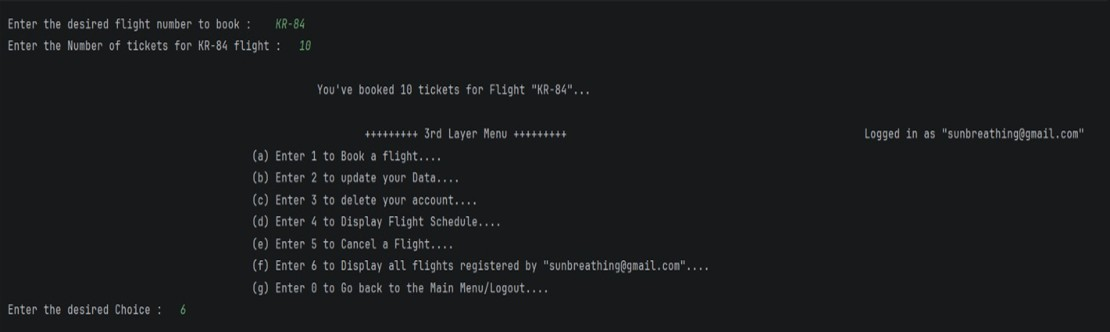
\includegraphics[width=\textwidth]{Figures/Picture5.jpg}
\caption{Ticket Booking Process}
\end{figure}
\vspace{-5pt}

As depicted in Figure~5.4, users can select a flight and enter the number of tickets required. The system processes the request and confirms the booking, ensuring real-time seat allocation and accuracy.

\FloatBarrier

\section{User Operations}

\subsection{User Menu Options}

After successful login, users are provided with multiple options to manage their activities within the system.

\begin{figure}[H]
\centering
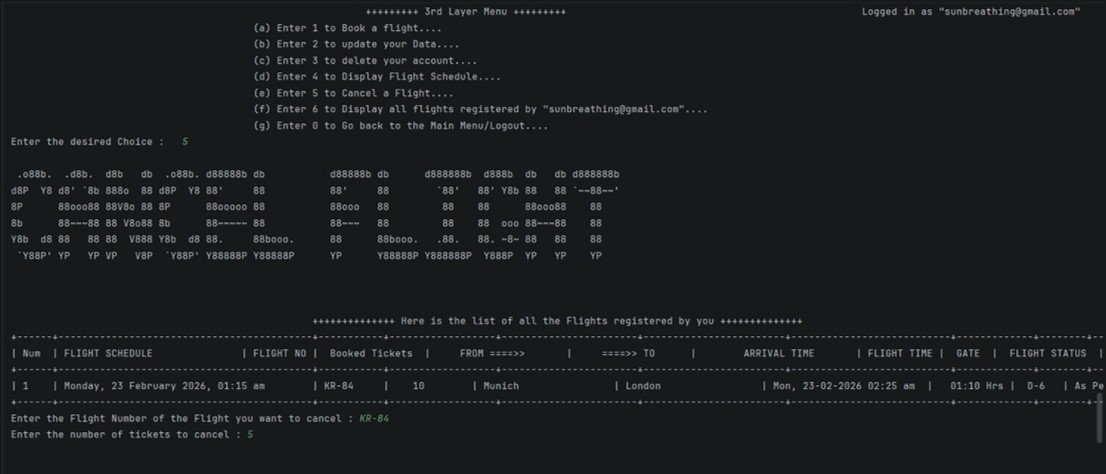
\includegraphics[width=\textwidth]{Figures/Picture7.jpg}
\caption{User Menu Interface}
\end{figure}
\vspace{-5pt}

Figure~5.5 illustrates the user menu, which includes options such as booking flights, updating personal details, viewing flight schedules, and canceling bookings. This enhances user control and flexibility.

\FloatBarrier

\subsection{Booking Details and Cancellation}

The system also provides functionality to view and manage booked tickets.

\begin{figure}[H]
\centering
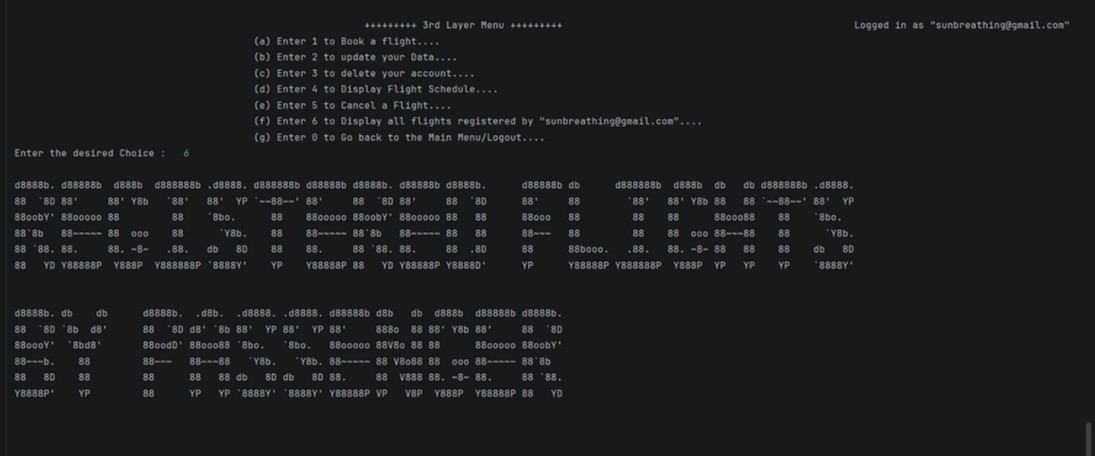
\includegraphics[width=\textwidth]{Figures/Picture8.jpg}
\caption{Booking Details and Cancellation}
\end{figure}
\vspace{-5pt}

As shown in Figure~5.6, users can view their booking details and cancel tickets if required. This feature ensures better management of reservations and improves overall user experience.
\bibitem{airline_uml}
\textbf{output :}
https://vscode.dev/github/recluzegeek/AirLineReservationSystem/blob/main
\FloatBarrier

\section{Summary}

This chapter demonstrated the implementation of the Airline Reservation System using various modules and console-based interfaces. The system effectively handles user interactions, flight management, and booking operations, ensuring accuracy, reliability, and ease of use.
\clearpage

\chapter{Results and Improvements}
\noindent\rule{\linewidth}{2pt}
\section{Introduction}

This chapter presents the results obtained from the implementation of the Airline Reservation System. It evaluates the performance of the system and discusses the improvements achieved over traditional manual methods. Additionally, it highlights possible enhancements that can be implemented in the future.

\section{Results}

The developed Airline Reservation System was successfully implemented using Java and tested with various user inputs. The system performs all core functionalities efficiently, including user registration, login, flight search, ticket booking, and cancellation.

\subsection{Functional Results}

The system was tested under different scenarios to verify its correctness and reliability. The following results were observed:

\begin{itemize}
\item The user registration module successfully stores user details without errors.
\item The login system correctly authenticates users based on valid credentials.
\item Flight details are displayed accurately with real-time seat availability.
\item Ticket booking is processed efficiently with proper seat allocation.
\item Cancellation of tickets updates the system records correctly.
\end{itemize}

\subsection{Performance Analysis}

The system demonstrates efficient performance in handling user operations. The response time for booking and cancellation operations is minimal, ensuring a smooth user experience. Since the system is console-based, it requires minimal system resources and performs efficiently even on low-end systems.

\subsection{Comparison with Existing System}

Compared to traditional manual reservation systems, the developed system offers several advantages:

\begin{itemize}
\item Reduces human errors in booking and record management.
\item Provides faster processing of reservations.
\item Ensures accurate and organized data storage.
\item Improves overall efficiency and user satisfaction.
\end{itemize}

\section{Improvements}

Although the current system meets basic requirements, several improvements can be made to enhance its functionality and usability.

\subsection{Graphical User Interface (GUI)}

The current system is console-based. A graphical user interface can be developed to make the system more interactive and user-friendly.

\subsection{Online Payment Integration}

The system can be enhanced by integrating secure online payment gateways to allow users to complete transactions digitally.

\subsection{Web-Based Application}

The system can be converted into a web-based application using technologies such as HTML, CSS, JavaScript, and frameworks like Spring Boot to allow access from anywhere.

\subsection{Real-Time Database Integration}

Currently, the system uses basic database operations. It can be improved by implementing real-time database updates and cloud-based storage for better scalability.

\subsection{Security Enhancements}

Additional security features such as encryption, authentication mechanisms, and role-based access control can be implemented to protect user data.

\section{Summary}

This chapter presented the results of the Airline Reservation System and demonstrated its effectiveness in handling booking operations. The system significantly improves efficiency compared to manual methods. Future enhancements can further expand the system’s capabilities and usability.
\clearpage

\chapter{Conclusion and Future Work}
\noindent\rule{\linewidth}{2pt}
\section{Conclusion}

The Airline Reservation System developed in this project successfully demonstrates the application of Object-Oriented Programming (OOP) concepts using Java. The system provides an efficient and reliable solution for managing airline reservations, including user registration, login, flight search, ticket booking, and cancellation.

The implementation of core OOP principles such as encapsulation, inheritance, polymorphism, and abstraction has ensured modularity and maintainability of the system. The system effectively reduces manual errors, improves data accuracy, and enhances the overall efficiency of reservation management.

Through the implementation and testing phases, the system has proven to be stable, user-friendly, and capable of handling basic airline booking operations. The console-based design ensures simplicity and ease of use while maintaining functional correctness.

Overall, the project demonstrates how software solutions can be used to automate real-world problems and improve operational efficiency in the airline industry.

\section{Future Work}
Although the system meets the primary requirements, there are several opportunities for future enhancements to further improve its functionality, usability, and overall performance. By incorporating advanced features and modern technologies, the system can be made more efficient, scalable, and user-friendly, thereby extending its applicability in real-world airline reservation scenarios.
\subsection{Graphical User Interface}

The current system is console-based. Developing a graphical user interface (GUI) using technologies such as JavaFX or Swing can make the system more interactive and user-friendly.

\subsection{Online Booking and Payment Integration}

The system can be extended to support online booking with secure payment gateway integration, enabling users to make real-time transactions.

\subsection{Web-Based and Mobile Application}

The application can be transformed into a web-based or mobile application using modern technologies, allowing users to access the system from anywhere at any time.

\subsection{Advanced Database Management}

Integration with advanced database systems and cloud storage can improve scalability, reliability, and real-time data processing.

\subsection{Security Enhancements}

Future improvements can include advanced security features such as data encryption, secure authentication mechanisms, and role-based access control to ensure data privacy and protection.

\section{Summary}

This chapter concludes the project by summarizing the achievements of the Airline Reservation System and outlining possible future enhancements. The system provides a strong foundation for further development and real-world deployment.
\clearpage
%%%%%%%%%%%%%%%% REFERENCES %%%%%%%%%%%%%%%%
\chapter*{References}
\addcontentsline{toc}{chapter}{References}

\begin{enumerate}
\small

\item \textbf{J. Bloch}, \textit{Effective Java}, 3rd ed., Addison-Wesley, 2018.\\
\textit{Available:} \url{https://www.oreilly.com/library/view/effective-java-3rd/9780134686097/}\\
\hspace*{1em}This book provides best practices for writing robust and efficient Java programs.\\
\hspace*{1em}It helped in understanding object-oriented principles used in system development.

\item \textbf{I. Sommerville}, \textit{Software Engineering}, 10th ed., Pearson, 2016.\\
\textit{Available:} \url{https://www.pearson.com/en-us/subject-catalog/p/software-engineering/P200000003354}\\
\hspace*{1em}This reference explains software development methodologies and system design concepts.\\
\hspace*{1em}It guided the overall structure and development approach of the project.

\item \textbf{E. Gamma et al.}, \textit{Design Patterns}, Addison-Wesley, 1994.\\
\textit{Available:} \url{https://www.oreilly.com/library/view/design-patterns-elements/0201633612/}\\
\hspace*{1em}This book introduces reusable object-oriented design patterns.\\
\hspace*{1em}It helped in implementing modular and scalable system architecture.

\item \textbf{T. H. Cormen et al.}, \textit{Introduction to Algorithms}, MIT Press, 2009.\\
\textit{Available:} \url{https://mitpress.mit.edu/9780262033848/introduction-to-algorithms/}\\
\hspace*{1em}This book covers fundamental algorithms used in software development.\\
\hspace*{1em}It supported efficient handling of data and operations in the system.

\item \textbf{S. Malik and P. Singh}, “Airline Reservation System Using Java,” IJCA, 2021.\\
\textit{Available:} \url{https://www.ijcaonline.org/archives/volume183/number12/31930-2021919902}\\
\hspace*{1em}This paper presents a Java-based airline reservation system design.\\
\hspace*{1em}It provided insights into implementing booking and management modules.

\item \textbf{R. Kumar and A. Sharma}, “Web-Based Airline Reservation Systems,” IJARCS, 2022.\\
\textit{Available:} \url{https://ijarcs.info/index.php/Ijarcs/article/view/6978}\\
\hspace*{1em}This study discusses web-based airline reservation approaches.\\
\hspace*{1em}It helped in understanding modern system requirements and scalability.

\item \textbf{M. Patel and K. Shah}, “Airline Reservation System Using OOP,” IJERT, 2023.\\
\textit{Available:} \url{https://www.ijert.org/research/airline-reservation-system-using-oop-IJERTV12IS050123.pdf}\\
\hspace*{1em}This paper focuses on using OOP concepts in airline systems.\\
\hspace*{1em}It supported the application of encapsulation and inheritance.

\item \textbf{D. Lee and H. Kim}, “Modern Airline Systems,” IEEE Access, 2024.\\
\textit{Available:} \url{https://ieeexplore.ieee.org/}\\
\hspace*{1em}This research highlights modern architectures for airline systems.\\
\hspace*{1em}It contributed to understanding system efficiency and performance.

\item \textbf{A. Verma and S. Gupta}, “Cloud-Based Airline Systems,” IJCC, 2025.\\
\textit{Available:} \url{https://www.inderscience.com/jhome.php?jcode=ijcc}\\
\hspace*{1em}This paper discusses cloud-based reservation systems.\\
\hspace*{1em}It provided ideas for scalability and future improvements.

\item \textbf{K. Reddy and V. Rao}, “Database in Airline Systems,” 2022.\\
\textit{Available:} \url{https://www.ijcsit.com/docs/Volume13/vol13issue02/ijcsit2022130205.pdf}\\
\hspace*{1em}This study focuses on database management techniques.\\
\hspace*{1em}It helped in designing structured and efficient data storage.

\item \textbf{P. Sharma}, “Object-Oriented Design in Java,” 2021.\\
\textit{Available:} \url{https://www.ijert.org/research/object-oriented-design-in-java-IJERTV10IS060456.pdf}\\
\hspace*{1em}This paper explains object-oriented programming concepts in Java.\\
\hspace*{1em}It supported implementation of modular system components.

\item \textbf{L. Wang}, “Cloud Reservation Systems,” IEEE, 2023.\\
\textit{Available:} \url{https://ieeexplore.ieee.org/}\\
\hspace*{1em}This research explores cloud-based reservation architectures.\\
\hspace*{1em}It provided insights into distributed system design.



\end{enumerate}
\end{document}